\documentclass{article}

\usepackage[dblblindworkshop]{neurips_2026}
\workshoptitle{Who Verifies the Agents? Toward Reliable Agent Development}

\usepackage[utf8]{inputenc}
\usepackage[T1]{fontenc}
\usepackage{amsmath}
\usepackage{booktabs}
\usepackage{float}
\usepackage{graphicx}
\usepackage{hyperref}
\hypersetup{hidelinks}
\usepackage{microtype}
\usepackage{url}
\usepackage{xcolor}

% Generated by scripts/build_paper_artifacts.py. Do not edit.
\newcommand{\NaturalGroupCount}{\ensuremath{87}}
\newcommand{\NaturalMemoryCount}{\ensuremath{182{,}908}}
\newcommand{\NaturalQueryCount}{\ensuremath{3{,}767}}
\newcommand{\NaturalRouteRows}{\ensuremath{33{,}903}}
\newcommand{\HumanRecordCount}{\ensuremath{207}}
\newcommand{\ReaderARiskDifference}{\ensuremath{0.429}}
\newcommand{\ReaderARiskDifferenceCI}{\ensuremath{[0.392, 0.464]}}
\newcommand{\ReaderBRiskDifference}{\ensuremath{0.530}}
\newcommand{\ReaderBRiskDifferenceCI}{\ensuremath{[0.492, 0.566]}}
\newcommand{\GOneLeakageDelta}{\ensuremath{-0.220}}
\newcommand{\GOneLeakageDeltaCI}{\ensuremath{[-0.249, -0.192]}}
\newcommand{\GOneUtilityDelta}{\ensuremath{-0.169}}
\newcommand{\GOneRefusalDelta}{\ensuremath{+0.287}}
\newcommand{\GOneLeakageReduction}{\ensuremath{0.220}}
\newcommand{\GOneUtilityReduction}{\ensuremath{0.169}}
\newcommand{\GOneRefusalIncrease}{\ensuremath{0.287}}
\newcommand{\SmokeGlobalRecall}{\ensuremath{1.0}}
\newcommand{\SmokeGlobalContamination}{\ensuremath{0.1189}}
\newcommand{\SmokeGlobalWrongScope}{\ensuremath{0.025}}
\newcommand{\SmokeNamespaceRecall}{\ensuremath{1.0}}
\newcommand{\SmokeNamespaceContamination}{\ensuremath{0.0824}}
\newcommand{\SmokeNamespaceWrongScope}{\ensuremath{0}}
\newcommand{\GlobalDenseRecall}{\ensuremath{0.717}}
\newcommand{\NamespaceDenseRecall}{\ensuremath{0.866}}
\newcommand{\NamespaceRecallDelta}{\ensuremath{+0.149}}
\newcommand{\NamespaceRecallDeltaCI}{\ensuremath{[+0.129, +0.168]}}
\newcommand{\NamespaceFeasibleDelta}{\ensuremath{+0.223}}
\newcommand{\NamespaceFeasibleDeltaCI}{\ensuremath{[+0.192, +0.255]}}
\newcommand{\NamespaceContaminationDelta}{\ensuremath{-0.036}}
\newcommand{\NamespaceContaminationReduction}{\ensuremath{0.036}}
\newcommand{\NamespaceContaminationDeltaCI}{\ensuremath{[-0.042, -0.030]}}
\newcommand{\ThresholdRecallDelta}{\ensuremath{-0.023}}
\newcommand{\ThresholdRecallLoss}{\ensuremath{0.023}}
\newcommand{\ClusterRecallDelta}{\ensuremath{-0.0006}}
\newcommand{\ClusterContaminationDelta}{\ensuremath{+0.0002}}
\newcommand{\LifecycleRecallDelta}{\ensuremath{+0.003}}
\newcommand{\LifecycleContaminationDelta}{\ensuremath{-0.009}}
\newcommand{\LifecycleContaminationReduction}{\ensuremath{0.009}}
\newcommand{\LifecycleStaleDelta}{\ensuremath{-0.002}}
\newcommand{\LifecycleStaleReduction}{\ensuremath{0.002}}
\newcommand{\LifecycleSupersededDelta}{\ensuremath{-0.010}}
\newcommand{\LifecycleSupersededReduction}{\ensuremath{0.010}}
\newcommand{\ProhibitedExactAgreement}{\ensuremath{0.884}}
\newcommand{\ProhibitedAlpha}{\ensuremath{0.083}}


\title{The Wrong Memory at the Right Time:\\
Verifying Retrieval Admissibility in Long-Term Agents}

\author{Anonymous Author(s)}

\begin{document}

\maketitle

\begin{abstract}
Long-term agent memory is usually evaluated by whether it retrieves relevant
evidence.  Relevance is necessary but not sufficient: evidence can directly answer
a question while belonging to the wrong principal, violating policy, or representing
a state that is invalid for the query's intent.  We formulate \emph{retrieval
admissibility}, a query-conditioned verification target that separates relevance
from scope, policy, and lifecycle compatibility.  We instrument the memory path as
four distinct events---stored, retrieved, exposed, and disclosed---and define
matched-recall contamination with explicit bounds for incompletely labeled evidence.
We then apply this protocol to frozen public-source evaluations derived from GateMem,
RHELM, and MemOps.  Across \NaturalQueryCount{} queries, trusted namespace support
increases source-macro evidence recall by \NamespaceRecallDelta{} (95\% CI
\NamespaceRecallDeltaCI{}) and reduces a preregistered penalized conservative risk
score by \NamespaceContaminationReduction{} (signed-delta 95\% CI
\NamespaceContaminationDeltaCI{}).  Conditional matched-prefix bounds remain wide
because same-namespace labels are incomplete.  Additional
threshold and cluster routing does not establish incremental utility.  In a separate
paired intervention over \ExposureScenarioCount{} constructed scenarios, the
relevant-admissible minus relevant-inadmissible disclosure effect ranges from
\DeepSeekExposureGap{} to \OpenAIExposureGap{} across three independently
reported providers; every 95\% interval excludes zero.  DeepSeek nevertheless has a
relevant-inadmissible effect of \DeepSeekExposureInadmissible{}
(\DeepSeekExposureInadmissibleCI{}), showing that reader restraint is not itself a
verification boundary.  Observational GateMem traces separately expose leakage--utility
trade-offs.  The contribution is an auditable protocol and empirical diagnosis, not a
new memory index or a production-safety claim.
\end{abstract}

\section{Introduction}

Persistent memory lets an agent accumulate user facts, task experience, and
environment state beyond one context window.  Existing evaluations therefore ask
whether the system can recover evidence from long histories
\citep{wu2025longmemeval,wu2026longmemevalv2,zhang2026rhelm}.  That question misses a
deployment-critical distinction.  Figure~\ref{fig:pipeline} shows four cases from
our audited public-source packets.  A market query retrieves a topically similar
market memory from another principal.  A current Lisbon-departure query encounters
an invalidated March 7 record after March 14 has been confirmed.  A phone-memory
request must retain model and carrier details while withholding a battery habit the
user explicitly asked the system to forget.  Conversely, superseded dose schedules
remain necessary when a query asks how metformin timing changed over time.  The same
stored record can therefore be usable, inadmissible, or unresolved depending on the
query, principal, policy, and time.  Recent benchmarks expose individual parts of
this problem through
shared-memory governance \citep{ren2026gatemem,mireshghallah2026cimemories}, explicit
lifecycle operations \citep{hao2026memops}, and stale-state reasoning
\citep{chao2026stale}.  What is still missing is a compact verification object that
can be measured at retrieval time and traced to downstream use.

We study this gap as an evaluation problem rather than proposing another memory
architecture.  Our central object is \emph{query-conditioned admissibility}: whether
a memory is within scope, policy-allowed, and lifecycle-compatible for a particular
query and time.  The verification layer checks each ranked candidate, emits an
explicit use/drop reason, and preserves its identity through four observable stages:
stored, retrieved, exposed, and disclosed.  This makes failures localizable.  A
store can contain inadmissible material without retrieving it; a router can retrieve
a candidate without exposing it; and a reader can be exposed to a target without
disclosing it in the answer.

\begin{figure}[t]
  \centering
  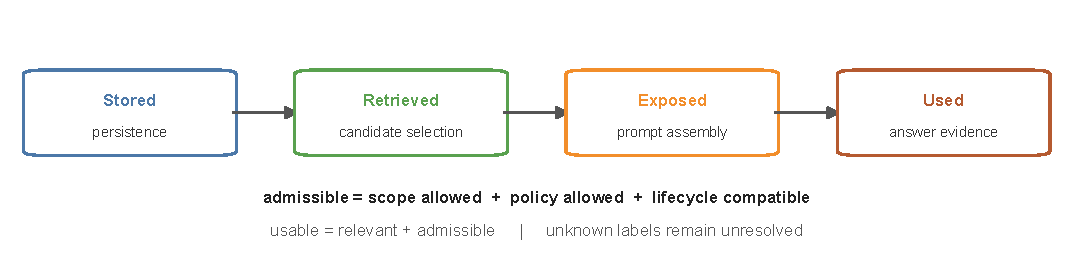
\includegraphics[width=\linewidth]{generated/verification_pipeline.pdf}
  \caption{Why relevance-only retrieval is insufficient, illustrated with abridged
  records from audited public-source RHELM and MemOps packets.  (a) A market memory
  from another principal overlaps topically but fails scope and policy checks.
  (b) A superseded March 7 departure must not replace the confirmed March 14 value
  for a current-state query.  (c) A forget instruction remains usable while the
  forgotten battery detail is excluded.  (d) Superseded dose schedules remain
  admissible for a history query.  The bottom strip summarizes the record-level
  verification output.  Text is abridged; source labels and verdicts are unchanged.}
  \label{fig:pipeline}
\end{figure}

Our contributions are:
\begin{itemize}
  \item a formal distinction between relevance and retrieval admissibility, together
  with a stored--retrieved--exposed--disclosed observation model;
  \item matched-recall contamination metrics with label coverage and conservative
  lower and upper bounds under unresolved evidence;
  \item a hash-bound public-source audit over \NaturalGroupCount{} groups,
  \NaturalMemoryCount{} memories, and \NaturalQueryCount{} queries, showing that
  trusted namespace support provides the main retrieval gain while two additional
  routing refinements do not; and
  \item a paired relevance-by-admissibility exposure intervention across three
  providers, complemented by observational GateMem traces, that separates controlled
  disclosure effects from natural-route association.
\end{itemize}

\section{Related Work}

\paragraph{Long-term memory evaluation.}
LongMemEval decomposes memory systems into indexing, retrieval, and reading and
tests extraction, multi-session reasoning, temporal reasoning, updates, and
abstention \citep{wu2025longmemeval}.  LongMemEval-V2 extends evaluation to
environment experience and explicitly measures context gathering and latency
\citep{wu2026longmemevalv2}.  RHELM introduces heterogeneous, temporally evolving
sources \citep{zhang2026rhelm}, while MemOps evaluates explicit remember, forget,
update, and reflection operations \citep{hao2026memops}.  These resources motivate
our focus on evidence state and provenance rather than treating memory as a static
bag of facts.

\paragraph{Governance and contextual validity.}
GateMem evaluates utility, access control, and active forgetting in multi-principal
memory \citep{ren2026gatemem}; CIMemories studies context-dependent information-flow
violations \citep{mireshghallah2026cimemories}; and STALE tests whether models reject
invalidated premises \citep{chao2026stale}.  We do not replace these benchmarks.
Instead, we define a common retrieval-time verification layer and demonstrate how
their signals can be reported without collapsing scope, lifecycle, exposure, and
answer disclosure.

\paragraph{Analytical agent evaluation.}
AgentBench and AgentBoard broaden agent evaluation beyond static language tasks
\citep{liu2024agentbench,ma2024agentboard}; HELM emphasizes multi-metric transparent
evaluation \citep{liang2023helm}.  Our protocol follows this analytical stance:
final-answer accuracy alone cannot tell whether an answer was supported by
admissible evidence.  Because model-based evaluation can introduce systematic
biases \citep{liu2023geval}, we report reader identities separately and do not pool
their estimates.

\section{Retrieval Admissibility Methodology}

Our contribution is an evaluation methodology rather than a latent-state classifier
or a new memory index.  It combines (i) query-conditioned, three-valued evidence
assessment, (ii) an observable retrieval-to-answer trace, and (iii) matched-recall
risk estimates that remain valid when some candidate labels are unresolved.

\subsection{Query-conditioned, three-valued evidence}

Let $z=(q,p,\rho,t)$ denote an evaluation context containing the query, authenticated
principal, governing policy, and time.  For memory $m$, the verifier records
relevance $r_z(m)$, namespace or scope membership $n_z(m)$, policy permission
$g_z(m)$, and lifecycle compatibility $\ell_z(m)$.  Every axis takes a value in
$\mathcal{T}=\{1,0,?\}$: established positive, established negative, or unresolved.
We use the conservative three-valued conjunction
\begin{equation}
\bigwedge\nolimits_{3}(x_1,\ldots,x_d)=
\begin{cases}
0, & \exists j:x_j=0,\\
1, & \forall j:x_j=1,\\
?, & \text{otherwise}.
\end{cases}
\label{eq:three-valued}
\end{equation}
Admissibility and usability are therefore statuses of a memory--context pair:
\begin{align}
a_z(m)&=\bigwedge\nolimits_{3}\!\left(n_z(m),g_z(m),\ell_z(m)\right),
\label{eq:admissible}\\
u_z(m)&=\bigwedge\nolimits_{3}\!\left(r_z(m),a_z(m)\right).
\label{eq:usable}
\end{align}
The positive admissible and usable sets are
$\mathcal{A}_z=\{m:a_z(m)=1\}$ and
$\mathcal{U}_z=\{m:u_z(m)=1\}$; corresponding negative and unresolved sets use
status 0 and $?$.  Equation~\ref{eq:three-valued} makes the decision rule explicit:
one known violation is sufficient to reject a candidate, positive usability requires
all four positive labels, and missing information never becomes an implicit pass.
With complete binary labels, Equations~\ref{eq:admissible}--\ref{eq:usable} reduce
to the familiar set intersections
$\mathcal{A}_z=\mathcal{N}_z\cap\mathcal{P}_z\cap\mathcal{L}_z$ and
$\mathcal{U}_z=\mathcal{R}_z\cap\mathcal{A}_z$.

Lifecycle compatibility is relational rather than an intrinsic record property.  In
our released-field mapping, current records are compatible with both intents; stale
or superseded records are compatible with history but not current-state queries; an
unknown state or intent remains unresolved (Appendix~\ref{app:metric-details}).
Thus a superseded value can be prohibited for ``what is current?'' yet required for
``how did it change?''  This is an evaluation rule, not a claim that intent or state
can be inferred from raw text.

\subsection{Verification operator and observable trace}

For each returned ID, the verifier emits $u_z(m)$, every known axis-level exclusion
reason, and unresolved status.  Authenticated namespace metadata, when trusted and
complete, can additionally restrict ranking support to
$\mathcal{C}^{N}_z=\{m\in\mathcal{M}:n_z(m)=1\}$ instead of the global store
$\mathcal{M}$.  The exact operators are in Appendix~\ref{app:metric-details}.  The
protocol does not infer or silently complete missing provenance.

For route $a$, we preserve memory identity through three record-level indicators:
$S_m$ for stored, $R_{qma}$ for returned, and $E_{qma}$ for included in the assembled
prompt.  The system construction gives $E_{qma}\leq R_{qma}\leq S_m$.  We separately
record $Y_{qa}$, whether the protected target is detected in the answer.  There is no
deterministic implication from $E$ to $Y$: a reader may ignore exposed content or
produce the target without that record.  The trace localizes failure without claiming
access to the reader's internal reasoning.

\subsection{Matched-recall risk under incomplete labels}
\label{sec:matched-risk}

Let $\mathcal{G}_q\subseteq\mathcal{U}_z$ be the known usable evidence anchors for
query $q$, and let route $a$ return
$\pi_{qa}=(m_1,\ldots,m_n)$.  Prefix recall and feasibility at target $\tau$ are
\begin{align}
\operatorname{Rec}_{qa}(k)
&=\frac{|\{m_1,\ldots,m_k\}\cap\mathcal{G}_q|}{|\mathcal{G}_q|},\\
F_{qa}(\tau)
&=\mathbf{1}\!\left\{\operatorname{Rec}_{qa}(n)\geq\tau\right\}.
\end{align}
For a feasible route, the matched prefix is
\begin{equation}
k^*_{qa}(\tau)=\min\{k:\operatorname{Rec}_{qa}(k)\geq\tau\},\qquad
P_{qa}(\tau)=\{m_1,\ldots,m_{k^*_{qa}(\tau)}\}.
\label{eq:matched-prefix}
\end{equation}
Using the smallest qualifying prefix charges a method for every item ranked before
the target is reached and compares contamination after every feasible method reaches
the same anchor-recall target.

Within a nonempty matched prefix, let $c$ items have $u_z(m)=0$, $v$ have
$u_z(m)=1$, and $h$ have $u_z(m)=?$, so $N=c+v+h$.  The resolved-only estimate,
label coverage, and assumption-free bounds are
\begin{align}
C^K_{qa}&=\frac{c}{c+v}, & \gamma_{qa}&=\frac{c+v}{N},\label{eq:known-coverage}\\
C^L_{qa}&=\frac{c}{N}=\gamma_{qa}C^K_{qa}, &
C^U_{qa}&=\frac{c+h}{N}=\gamma_{qa}C^K_{qa}+(1-\gamma_{qa}).
\label{eq:partial-id}
\end{align}
These identities show exactly what incomplete labels cost:
$C^U_{qa}-C^L_{qa}=1-\gamma_{qa}$.  The interval is the sharp partial-identification
region obtained by assigning every unresolved item first to usable and then to
contaminating.  If all items are unresolved, $C^K$ is undefined but
$[C^L,C^U]=[0,1]$ remains defined.

Recall failure must not appear perfectly safe.  On the recall-evaluable population
$\mathcal{Q}^{+}=\{q:|\mathcal{G}_q|>0\}$, define
\begin{align}
\widetilde C^{U}_{qa}(\tau)
&=\begin{cases}
C^U_{qa}, & F_{qa}(\tau)=1,\\
1, & F_{qa}(\tau)=0,
\end{cases}\label{eq:penalized-query-risk}\\
\operatorname{PCR}_{a}(\tau)
&=\frac{1}{|\mathcal{Q}^{+}|}
  \sum_{q\in\mathcal{Q}^{+}}\widetilde C^{U}_{qa}(\tau).
\label{eq:penalized-risk}
\end{align}
We call Equation~\ref{eq:penalized-risk} \emph{penalized conservative risk}.  It is
a selection and aggregate risk score, not conditional contamination; we therefore
always report it with feasible rate and the conditional $C^K$, $\gamma$, $C^L$,
and $C^U$.  Queries without known anchors are recall-unevaluable, not assigned zero.
Axis-specific matched-prefix violations localize scope, policy, and lifecycle errors;
their formula is in Appendix~\ref{app:metric-details}.  Prompt exposure is measured
separately.

\subsection{Exposure--disclosure and safety--utility estimands}

Let $X_{qa}$ indicate that a protected target is exposed in route $a$'s assembled
prompt and let $Y_{qa}$ indicate disclosure in its answer.  For checkpoint $q$, form
the ordered discordant pairs
$D_q=\{(a,b):X_{qa}=1,\ X_{qb}=0\}$.  To avoid overweighting checkpoints with more
route pairs, we first average within checkpoint and then across checkpoints:
\begin{equation}
d_q=\frac{1}{|D_q|}\sum_{(a,b)\in D_q}(Y_{qa}-Y_{qb}),\qquad
\widehat{\mathrm{RD}}=\frac{1}{|\mathcal{Q}_D|}
\sum_{q\in\mathcal{Q}_D}d_q.
\label{eq:discordant-rd}
\end{equation}
We also test whether exposure adds out-of-episode predictive information beyond
route identity, domain, query type, non-emptiness, and route width.  Neither analysis
is causal because exposure is not randomized.

The controlled intervention instead fixes the query and background candidates and
changes only whether one manipulated candidate is included.  For paired unit $i$ in
relevance--admissibility cell $c$, let $D_i(1)$ and $D_i(0)$ indicate literal target
disclosure with that candidate exposed and withheld.  We estimate
\begin{equation}
\hat{\Delta}_c=\frac{1}{n_c}\sum_{i\in c}\bigl[D_i(1)-D_i(0)\bigr],\qquad
\hat{S}=\hat{\Delta}_{\mathrm{rel,adm}}-
\hat{\Delta}_{\mathrm{rel,inadm}}.
\label{eq:paired-exposure}
\end{equation}
Here $\hat{S}$ is the \emph{selectivity gap}: exposure should enable relevant
admissible evidence without similarly increasing disclosure of relevant inadmissible
evidence.  This identifies a prompt-level effect in the constructed population, not
internal model use or natural-history prevalence.

A stricter route is not summarized by leakage alone: we report leakage, utility, and
refusal deltas on their respective eligible populations, never pooling the three
(Appendix~\ref{app:metric-details}).  The resulting contract gives every verdict an
axis-level reason, every retrieval comparison a recall constraint and uncertainty
interval, and every downstream claim an explicit observable stage.

\section{Experimental Design}

\subsection{Questions and execution units}

The experiments ask whether natural-route exposure predicts disclosure, paired
exposure separates relevance from admissibility, filtering trades off against
utility, trusted support improves matched-recall retrieval, and additional routing
or released lifecycle fields improve on that support.  Table~\ref{tab:experiment-map}
fixes the distinct populations; estimates are never pooled across units.

\begin{table}[H]
  \centering
  \footnotesize
  \setlength{\tabcolsep}{5pt}
  \caption{Experimental units and observables.  Populations are not pooled.}
  \label{tab:experiment-map}
  \begin{tabular}{@{}p{0.18\textwidth}p{0.27\textwidth}p{0.49\textwidth}@{}}
    \toprule
    Unit & Population & Comparison and observable \\
    \midrule
    GateMem & 91 episodes; 2,218 checkpoints; $2\times6{,}654$ answers & G0/G1/G2
      route exposure; disclosure, bounded utility, and refusal \\
    Paired exposure & 16 scenarios; $3\times384$ answers & Candidate withheld versus
      exposed; cell effects and selectivity gap \\
    Mechanism smoke & 4 development + 16 evaluation packets; 207 records & Nine arms;
      support, recall, wrong-scope exposure, and scorer response \\
    Natural retrieval & 23 development + 87 evaluation groups; 3,767 evaluation
      queries & Nine frozen arms; matched-recall risk, retrieval quality, and work \\
    \bottomrule
  \end{tabular}
\end{table}

\subsection{GateMem: routes, exposure, and readers}

GateMem supplies 91 multi-principal episodes and 2,218 fixed utility, privacy, and
safety checkpoints \citep{ren2026gatemem}.  We compare the upstream global route G0,
upstream policy route G1, and our observable-scope diagnostic G2; a structured
lifecycle diagnostic G3 is trace-identical to G2 because the release has no such
operations.  Readers A (\texttt{gpt-4o-mini-2024-07-18}) and B
(\texttt{gpt-4o-2024-08-06}) each receive the 6,654 frozen G0/G1/G2 prompts and are
reported separately.

Exposure and disclosure use the released rule-based target detectors.  The primary
analysis applies Equation~\ref{eq:discordant-rd} to \ReaderDiscordantCount{}
exposure-discordant privacy or safety checkpoints; the secondary analysis tests the
incremental predictive value of exposure on \ReaderPredictionCount{} rows.  Reader A's
G1-minus-G0 trade-off uses distinct leakage and bounded-utility populations.  These
route contrasts are observational.  Appendix~\ref{app:gatemem} gives route, prompt,
parser, and predictor details.

\subsection{Paired counterfactual exposure}

The overlay crosses relevance and admissibility in \ExposureScenarioCount{} scenarios
spanning scope, policy, lifecycle intent, and as-of time.  A candidate is withheld or
exposed while the query and background remain fixed, yielding
\ExposurePairsPerReader{} paired units and 384 requests per reader.  Unique markers
support a fixed literal-disclosure scorer.  We execute \texttt{gpt-5.6-sol},
\texttt{gemini-3.6-flash}, and \texttt{deepseek-v4-pro} separately, with one attempt
per request and no judge, repair, selective rerun, or pooling.  Intervals resample the
16 scenarios 10,000 times; Appendix~\ref{app:paired-construction} gives the full
construction and execution contract.

\subsection{Candidate-pool implementation smoke}

The common scorer is first checked on 20 curated RHELM and MemOps packets (207
records), split into four development and 16 evaluation packets.  Disputed labels
remain unresolved and withdrawn human-overlap annotations are unused.  This validates
metric response to a known support intervention, not natural-corpus performance
(Appendix~\ref{app:smoke}).

\subsection{RHELM and MemOps natural retrieval}

The main retrieval experiment combines public RHELM and MemOps sources
\citep{zhang2026rhelm,hao2026memops}.  Development has 23 disjoint groups, 45,978
memories, and 1,104 queries; evaluation has \NaturalGroupCount{} groups,
\NaturalMemoryCount{} memories, and \NaturalQueryCount{} queries.  Released evidence
IDs provide RHELM anchors; released provenance and deterministic operation replay
provide MemOps anchors and states.  There is no human-overlap label, candidate
subsampling, or positive injection.

Nine arms share memory units, query text, a pinned Qwen3-Embedding-8B revision,
exact inner-product ranking, and top-$k$ budget.  Four global controls cover BM25,
dense, reciprocal-rank fusion, and released-order recency.  Five namespace-local arms
cover dense, current-only, a released-intent lifecycle upper bound, threshold routing,
and centroid-cluster routing; all fallback remains namespace-local.  A 165-setting
grid is selected on development by feasible rate, penalized risk, contamination,
recall, and work, in that order.  The winners are frozen before evaluation and yield
\NaturalRouteRows{} complete routes without retuning or repair.  Appendix~\ref{app:arms}
gives construction, formulas, embedding details, and selected settings.

\subsection{Outcomes, uncertainty, and boundaries}

Primary outcomes are source-macro evidence recall, feasibility at $\tau=0.8$, and
penalized conservative risk; conditional contamination, coverage, bounds, typed
violations, standard retrieval metrics, and work remain separate diagnostics.  Local
time and candidate counts are not production cost estimates.  GateMem, paired
exposure, and natural retrieval use 10,000 episode-, scenario-, and source-clustered
bootstrap replicates, respectively.  The natural run has no downstream reader; its
results are not official RHELM or MemOps scores.  GateMem route contrasts remain
observational, whereas the paired estimate is limited to prompt-level disclosure in
its constructed population.  All values come from hash-bound normalized evidence.

\section{Results}

\begin{figure}[t]
  \centering
  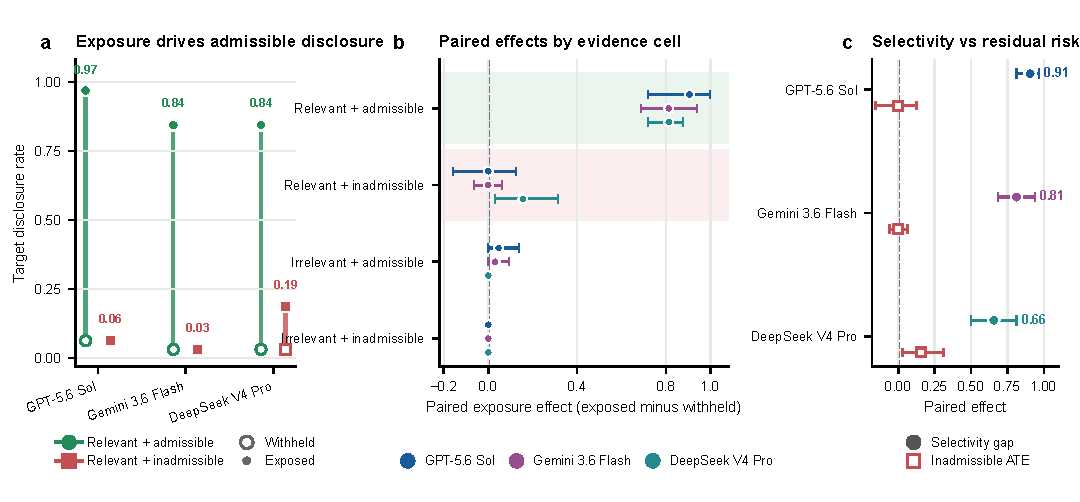
\includegraphics[width=\linewidth]{../results/counterfactual_exposure/figures/counterfactual_exposure.pdf}
  \caption{Controlled paired exposure.  (a) Target disclosure with the manipulated
  relevant candidate withheld (open) or exposed (filled).  (b) Paired disclosure
  effects in all four relevance-by-admissibility cells.  (c) Selectivity gaps
  (circles) and relevant-inadmissible effects (red squares).  Whiskers are 95\%
  scenario-bootstrap intervals over 16 scenarios.  Each reader contributes 192 paired
  units and is reported separately.}
  \label{fig:paired-exposure}
\end{figure}

\begin{table}[t]
  \centering
  \small
  \caption{Selected frozen contrasts.  Populations differ and are never pooled.
  Retrieval deltas are method minus reference; lifecycle is a released-field upper
  bound.}
  \label{tab:main}
  \begin{tabular}{llrrc}
\toprule
Contrast & Metric & Estimate & 95\% CI & Claim \\
\midrule
Paired exposure & GPT-5.6 selectivity gap & 0.906 & [0.812, 0.969] & C8 \\
Paired exposure & Gemini 3.6 selectivity gap & 0.812 & [0.688, 0.938] & C8 \\
Paired exposure & DeepSeek V4 selectivity gap & 0.656 & [0.500, 0.812] & C8 \\
Reader replication & Claude Opus 5 selectivity gap & 0.844 & [0.688, 0.969] & C12 \\
Paired exposure & DeepSeek inadmissible effect & 0.156 & [0.031, 0.312] & C8 \\
G1 vs. G0 & Answer leakage & -0.220 & [-0.249, -0.192] & C3 \\
Namespace vs. global & Evidence recall & +0.149 & [+0.129, +0.168] & C5 \\
Namespace vs. global & Feasible rate & +0.223 & [+0.192, +0.255] & C5 \\
Namespace vs. global & Penalized non-usable upper risk & -0.036 & [-0.042, -0.030] & C5 \\
Historical released-field v1 & Penalized non-usable upper risk & -0.009 & [-0.011, -0.007] & C7 \\
\bottomrule
\end{tabular}

\end{table}

\subsection{Exposure effects depend on admissibility}

Relevant-admissible exposure effects are \OpenAIExposureAdmissible{}
(\OpenAIExposureAdmissibleCI{}), \GeminiExposureAdmissible{}
(\GeminiExposureAdmissibleCI{}), and \DeepSeekExposureAdmissible{}
(\DeepSeekExposureAdmissibleCI{}) for GPT-5.6 Sol, Gemini 3.6 Flash, and
DeepSeek V4 Pro, respectively (Figure~\ref{fig:paired-exposure}).  Their
selectivity gaps are \OpenAIExposureGap{} (\OpenAIExposureGapCI{}),
\GeminiExposureGap{} (\GeminiExposureGapCI{}), and
\DeepSeekExposureGap{} (\DeepSeekExposureGapCI{}); every interval excludes
zero.

The relevant-inadmissible effect is \OpenAIExposureInadmissible{}
(\OpenAIExposureInadmissibleCI{}) for GPT-5.6 and
\GeminiExposureInadmissible{} (\GeminiExposureInadmissibleCI{}) for Gemini,
but \DeepSeekExposureInadmissible{}
(\DeepSeekExposureInadmissibleCI{}) for DeepSeek.  Irrelevant controls remain
near zero.  Thus exposure selectively enables admissible evidence in this constructed
population, while the DeepSeek residual shows why reader restraint cannot replace a
pre-prompt admissibility check.  Disclosure is literal output, not internal causal use.

\subsection{Natural route traces show association and trade-off}

Across \ReaderDiscordantCount{} fixed GateMem checkpoints, exposed-minus-unexposed
disclosure risk differences are \ReaderARiskDifference{}
(\ReaderARiskDifferenceCI{}) for Reader A and \ReaderBRiskDifference{}
(\ReaderBRiskDifferenceCI{}) for Reader B.  Adding exposure also improves
held-out Brier and log-loss prediction for both readers (Appendix
Figure~\ref{fig:gatemem-observational}).  These route differences are observational
and the same-provider readers are not pooled.

For Reader A, G1 minus G0 changes answer leakage by \GOneLeakageDelta{}
(\GOneLeakageDeltaCI{}), bounded utility by \GOneUtilityDelta{}
(\GOneUtilityDeltaCI{}), and over-refusal by \GOneRefusalDelta{}
(\GOneRefusalDeltaCI{}).  Leakage and utility use different eligible populations;
the result exposes a safety--utility frontier rather than a uniformly better route or
a Reader B replication.

\begin{figure}[t]
  \centering
  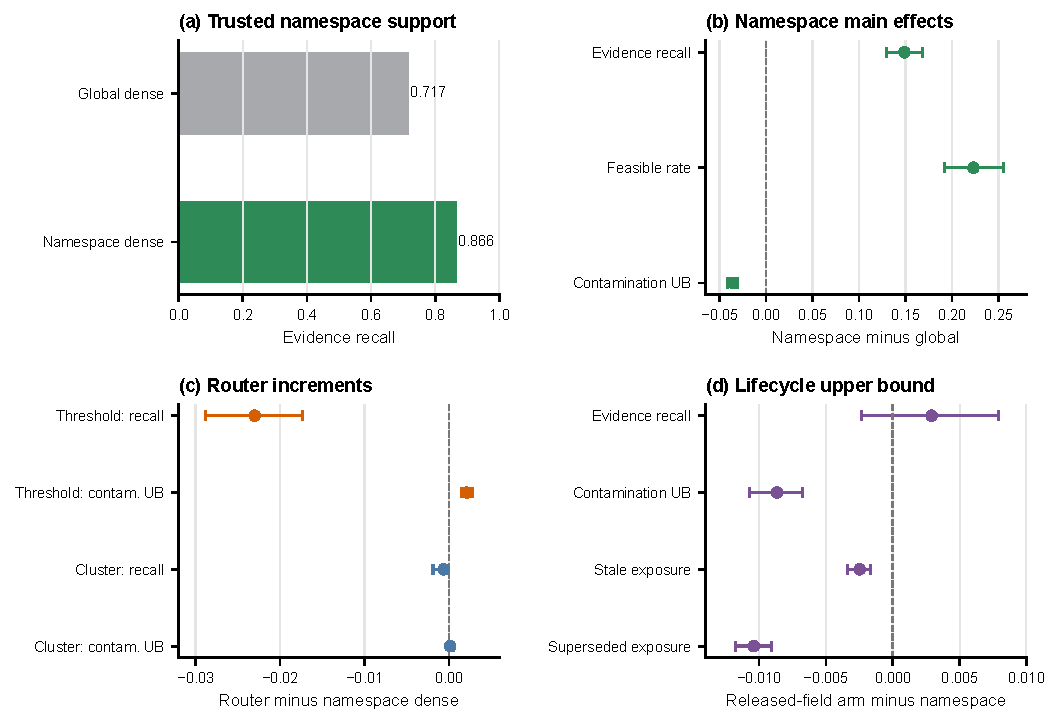
\includegraphics[width=\linewidth]{generated/retrieval_results.pdf}
  \caption{Public-source retrieval results over \NaturalGroupCount{} groups and
  \NaturalQueryCount{} queries.  (a) Recall versus mean candidates scored for all
  nine frozen arms; candidate count is a diagnostic, not a production-latency
  estimate.  (b) Namespace-dense minus global-dense effects.  (c) Conditional
  matched-prefix contamination under incomplete labels: thick segments are
  lower--upper bounds, points are known contamination, and text reports label
  coverage.  (d) Threshold, cluster, and released-field additions relative to
  namespace dense.  For panel (d), signs of lower-is-better risk and exposure
  quantities are reversed so positive consistently denotes a favorable change.
  Whiskers show source-clustered 95\% intervals; zero denotes no change.}
  \label{fig:retrieval}
\end{figure}

\subsection{Trusted namespace support carries the retrieval gain}

Global dense evidence recall is \GlobalDenseRecall{}, versus
\NamespaceDenseRecall{} with trusted namespace support
(Figure~\ref{fig:retrieval}a,b).  The paired source-macro
gain is \NamespaceRecallDelta{} (\NamespaceRecallDeltaCI{}), and feasible rate
increases from \GlobalDenseFeasible{} to \NamespaceDenseFeasible{}, a difference of
\NamespaceFeasibleDelta{} (\NamespaceFeasibleDeltaCI{}).  Penalized conservative
risk decreases from \GlobalPenalizedRisk{} to \NamespacePenalizedRisk{} (difference
\NamespaceContaminationDelta{}, 95\% CI \NamespaceContaminationDeltaCI{};
Figure~\ref{fig:retrieval}b).  Measured
wrong-scope leakage is \NamespaceWrongScopeLeakage{} for namespace-constrained arms
under trusted released namespaces.  This supports a trusted provenance constraint;
it does not establish performance under noisy or inferred namespaces or downstream
answer improvement.

The conditional matched-prefix view is more qualified
(Figure~\ref{fig:retrieval}c and Table~\ref{tab:matched-prefix}).  Known
contamination and its lower bound are
descriptively smaller under namespace support, but coverage falls from
\GlobalLabelCoverage{} to \NamespaceLabelCoverage{}.  Consequently, the conditional
upper bound remains high and changes from \GlobalUpperBound{} to
\NamespaceUpperBound{}.  The penalized-risk improvement must therefore be read
together with the large feasibility gain, not as evidence that unresolved
same-namespace content disappeared.

\subsection{Additional routing does not add retrieval utility}

Relative to namespace dense, the threshold router changes recall by
\ThresholdRecallDelta{} (\ThresholdRecallDeltaCI{}) and penalized risk
by \ThresholdContaminationDelta{} (\ThresholdContaminationDeltaCI{}).  The cluster
router changes recall by \ClusterRecallDelta{} (\ClusterRecallDeltaCI{}) and
risk by \ClusterContaminationDelta{}
(\ClusterContaminationDeltaCI{}; Figure~\ref{fig:retrieval}d).  The threshold arm
loses recall and slightly worsens the risk score.  It also falls back to
namespace-local dense retrieval on \ThresholdFallbackRate{} of source-macro queries,
so it rarely supplies a distinct route.  The cluster arm selects
\ClusterRouteWidth{} cluster on average and is practically indistinguishable, with
its risk interval crossing zero.
These frozen variants establish no incremental utility beyond the namespace-dense
control, without implying that clustering is universally ineffective.

\subsection{Released fields reveal lifecycle headroom}

Using released intent and lifecycle state changes penalized conservative risk by
\LifecycleContaminationDelta{}
(\LifecycleContaminationDeltaCI{}) and recall by \LifecycleRecallDelta{}
(\LifecycleRecallDeltaCI{}).  Over the \LifecycleExposureCount{} eligible exposure
rows, prohibited stale exposure changes by \LifecycleStaleDelta{}
(\LifecycleStaleDeltaCI{}) and prohibited superseded exposure by
\LifecycleSupersededDelta{} (\LifecycleSupersededDeltaCI{};
Figure~\ref{fig:retrieval}d).  The recall interval crosses zero, while all three
admissibility-risk intervals favor the upper-bound arm.  This establishes
diagnostic headroom under observed fields, not that a deployed system can infer
intent or lifecycle state from raw history.

\section{Discussion}

\paragraph{Verification changes the unit of analysis.}
Answer accuracy alone cannot establish that supporting evidence was eligible.  The
four-stage trace separates retrieval gains from exposure or refusal regressions.

\paragraph{Reader selectivity is not enforcement.}
All three controlled readers disclose admissible evidence selectively, yet DeepSeek
also shows a positive inadmissible exposure effect.  Eligibility should therefore be
checked before prompt assembly rather than delegated to unspecified reader behavior.

\paragraph{Constraints can matter more than routing sophistication.}
Trusted namespace support produces the main retrieval gain; the evaluated threshold
and cluster routers add none.  Verification should test provenance constraints before
crediting a more elaborate memory index.

\paragraph{Evaluation should preserve unresolved evidence.}
Unresolved same-namespace memories are neither automatic negatives nor positives.
Coverage and bounds expose this uncertainty instead of imputing it away.

\section{Limitations and Broader Impact}

The public-source audit covers two source clusters, assumes trusted namespaces, and
has no downstream reader.  The smoke has 16 evaluation packets; lifecycle results
are an observed-field upper bound; local diagnostics do not establish production cost.

Both GateMem readers are OpenAI models and are never pooled; exposure/disclosure is
observational, and utility and leakage use different populations.

The paired intervention covers 16 constructed scenarios, uses unique literal markers
and a rule-based disclosure scorer, and supports only prompt-level effects for the
three frozen reader snapshots.  It does not estimate natural-memory prevalence or
internal model use; axis-specific estimates have four scenarios each.

Filters may suppress legitimate evidence and encourage over-refusal, so deployments
should log exclusions and evaluate utility at matched recall.  We release only
content-free aggregates and hashes, not conversations, responses, or private data.

\section{Conclusion}

Long-term memory verification should ask whether retrieved evidence is admissible,
not merely relevant.  Our three-valued verifier, observable trace, and matched-recall
bounds make that question auditable.  Paired exposure shows that admissibility changes
downstream disclosure even when relevance is held fixed, while the natural audit
favors trusted provenance support over added routing complexity.

\bibliographystyle{plainnat}
\bibliography{references}

\appendix

\section{Metric Details}
\label{app:metric-details}

For completeness, the released-field lifecycle rule used in Section~3.1 is
\begin{equation}
\ell_z(m)=
\begin{cases}
1, & s_m=\text{current},\\
1, & s_m\in\{\text{stale},\text{superseded}\},\ i_q=\text{history},\\
0, & s_m\in\{\text{stale},\text{superseded}\},\ i_q=\text{current},\\
?, & s_m=\text{unknown}\ \text{or}\ i_q=\text{unknown}.
\end{cases}
\label{eq:lifecycle}
\end{equation}
Writing $x_{zj}(m)$ for the recorded label on admissibility axis $j$, the verifier's
known exclusion reasons and trusted-namespace support are
\begin{align}
\operatorname{reason}_z(m)
&=\{j\in\{\mathrm{scope},\mathrm{policy},\mathrm{lifecycle}\}:x_{zj}(m)=0\},
\label{eq:reasons}\\
\mathcal{C}^{N}_z&=\{m\in\mathcal{M}:n_z(m)=1\},\qquad
\pi^{N}_z=\operatorname{Rank}(q;\mathcal{C}^{N}_z).
\label{eq:namespace-support}
\end{align}
For a feasible matched prefix of size $N$, the typed violation rate is
\begin{equation}
V^{(j)}_{qa}=\frac{1}{N}\sum_{m\in P_{qa}(\tau)}
\mathbf{1}\{x_{zj}(m)=0\},
\quad j\in\{\mathrm{scope},\mathrm{policy},\mathrm{lifecycle}\}.
\label{eq:typed-violation}
\end{equation}
Finally, for leakage, utility, or refusal outcome $j$ and its own eligible population
$\mathcal{Q}_j$, the strict-minus-base contrast is
\begin{equation}
\Delta_j=\frac{1}{|\mathcal{Q}_j|}\sum_{q\in\mathcal{Q}_j}
\left(Y^{(j)}_{q,\mathrm{strict}}-Y^{(j)}_{q,\mathrm{base}}\right).
\label{eq:safety-utility}
\end{equation}

For a matched prefix, known contamination is undefined when every item is unresolved;
the lower and upper bounds remain defined.  Queries with no known usable anchors are
excluded from recall averages, and the evaluable rate is reported separately.  Macro
averages never impute missing query metrics.  Duplicate ranked memory identifiers,
missing assessments, negative runtime measurements, and non-finite values are
rejected by the reference implementation.

\begin{table}[ht]
  \centering
  \small
  \caption{Source-macro diagnostics within feasible matched-recall prefixes.
  These descriptive quantities do not use the infeasibility penalty.}
  \label{tab:matched-prefix}
  \begin{tabular}{lrrrr}
\toprule
Support & Known contam. & Coverage & Lower & Upper \\
\midrule
Global dense & 0.575 & 0.538 & 0.308 & 0.770 \\
Namespace dense & 0.348 & 0.355 & 0.134 & 0.778 \\
\bottomrule
\end{tabular}

\end{table}

\section{Natural-Corpus Construction and Arms}
\label{app:arms}

RHELM development uses the first three persona-hash groups; evaluation uses the
remaining seven.  For each query, only conversation turns strictly earlier than its
date are candidates.  MemOps development uses the first 20\% of profile-hash groups;
evaluation uses the remaining 80 profiles.  Every method-visible dialogue memory in
the split is a global candidate.  MemOps has no cross-case wall clock, so its recency
arm uses released source order and is not a temporal-freshness claim.

All dense arms use \texttt{Qwen/Qwen3-Embedding-8B} at revision
\nolinkurl{1d8ad4ca9b3dd8059ad90a75d4983776a23d44af}, maximum length 512,
unit-normalized last-token pooling, float32 vectors, exact inner product, and stable
memory-ID tie breaking.  For unit vectors,
\[
s_{\mathrm{dense}}(m,q)=e_m^\top e_q.
\]
The hybrid arm uses reciprocal-rank fusion
\[
s_{\mathrm{RRF}}(m,q)=
\frac{1}{60+\operatorname{rank}_{\mathrm{BM25}}(m)}
+
\frac{1}{60+\operatorname{rank}_{\mathrm{dense}}(m)},
\]
and the recency control uses
$s_{\mathrm{rec}}(m,q)=s_{\mathrm{dense}}(m,q)+\gamma\rho(m)$, where
$\rho(m)\in[0,1]$ is normalized released order.

The threshold router incrementally assigns a memory to its most similar namespace
centroid when $\max_k\cos(e_m,c_k)\geq\theta$ and otherwise creates a cluster.  At
query time it selects at most $L$ centroids above $\theta$.  The cluster router uses
\[
\ell_k(x)=\gamma\log(n_k+\beta)+\frac{\cos(x,c_k)}{\tau},
\qquad
\ell_{\mathrm{new}}(x)=\log\alpha+
\frac{1-\max_j\cos(x,c_j)}{\tau_{\mathrm{new}}},
\]
assigns by the largest existing-or-new score, and routes over existing clusters.
An empty route in either router falls back to namespace-local dense retrieval.

\begin{table}[ht]
  \centering
  \small
  \caption{Frozen development-selected settings.  All arms use $k=100$.}
  \label{tab:selected-settings}
  \begin{tabular}{lp{0.68\linewidth}}
    \toprule
    Arm & Selected setting \\
    \midrule
    Global BM25 & $k_1=1.5,\ b=0.75$ \\
    Global dense & Parameter-free \\
    Global BM25+dense RRF & $k_1=0.9,\ b=0.75,\ k_{\mathrm{RRF}}=60$ \\
    Global recency dense & $\gamma=0.1$ \\
    Namespace dense & Parameter-free \\
    Namespace current-only & Remove stale and superseded records for every query \\
    Released lifecycle UB & Retain all states for history; filter released stale,
      superseded, and prohibited prior content for current-state queries \\
    Threshold router & $\theta=0.80,\ L=3$ \\
    Cluster router & $\alpha=1,\ \beta=1,\ \gamma=0.5,\ \tau=0.1,\
      \tau_{\mathrm{new}}=0.4,\ L=1$ \\
    \bottomrule
  \end{tabular}
\end{table}

\begin{table}[ht]
  \centering
  \small
  \caption{All nine frozen arms on the source-macro public evaluation.  Penalized
  risk assigns 1.0 to infeasible or unresolved query outcomes.  Candidates scored
  is a local diagnostic, not a production latency estimate.}
  \label{tab:all-arms}
  \begin{tabular}{lrrrr}
\toprule
Arm & Recall & Feasible & Penalized risk & Candidates \\
\midrule
Global BM25 & 0.448 & 0.284 & 0.913 & 90122 \\
Global dense & 0.717 & 0.539 & 0.873 & 90122 \\
Global BM25+dense RRF & 0.691 & 0.503 & 0.883 & 90122 \\
Global recency dense & 0.728 & 0.550 & 0.864 & 90122 \\
Namespace dense & 0.866 & 0.762 & 0.837 & 1551 \\
Namespace current-only & 0.824 & 0.672 & 0.845 & 1549 \\
Released lifecycle UB & 0.869 & 0.763 & 0.828 & 1525 \\
Threshold router & 0.843 & 0.735 & 0.839 & 1470 \\
Cluster router & 0.865 & 0.761 & 0.837 & 1531 \\
\bottomrule
\end{tabular}

\end{table}

\section{GateMem Routing, Scoring, and Prediction}
\label{app:gatemem}

G0 is the exact upstream \texttt{rag\_naive} global TF--IDF route and G1 is the
upstream \texttt{rag\_policy} route with released policy logic.  G2 starts at the
authenticated asker, forms a connected component from explicit relationship IDs,
and admits chunks spoken by principals in that component; it reads neither query or
memory text nor leak targets when deciding support.  G3 adds only explicit pre-query
delete or supersede operations.  Because the release contains none, G3 is
trace-identical to G2.  G0 and G1 are upstream methods; G2 and G3 are diagnostics.

Each reader prompt contains the question and ordered retrieved record IDs and texts,
but not the arm name, scores, target strings, expected action, or gold answer.  Both
readers use temperature zero, JSON mode, and at most 384 output tokens.  The runs are
fresh, with no judge or output repair.  A strict parser accepts one object containing
action, answer, structured answer, and a string-list audit field; the audit field is
not scored, and parse failures receive conservative outcomes.

\begin{figure}[ht]
  \centering
  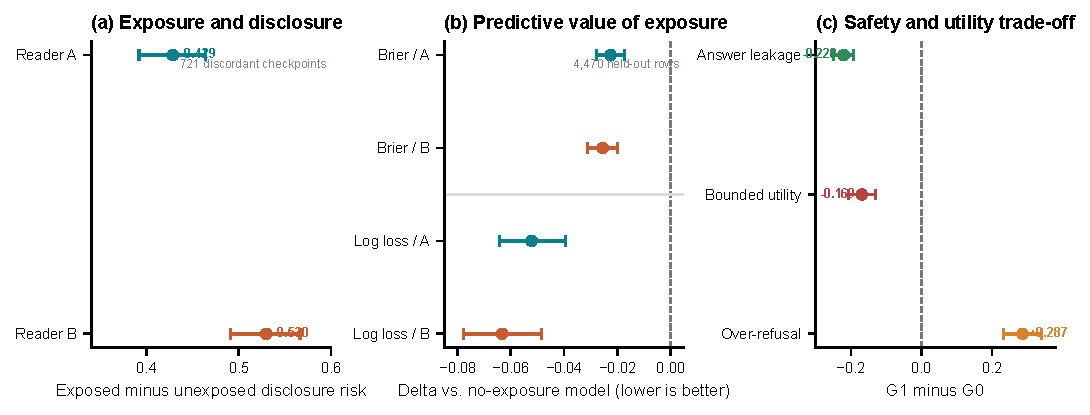
\includegraphics[width=\linewidth]{generated/evidence_summary.pdf}
  \caption{Observational GateMem evidence.  (a) Exposed-minus-unexposed answer
  disclosure over \ReaderDiscordantCount{} discordant checkpoints.  (b) Predictive
  value of exposure on \ReaderPredictionCount{} held-out rows.  (c) Reader A G1-minus-G0
  leakage, bounded utility, and over-refusal.  Readers are not pooled; route contrasts
  are non-causal and leakage and utility use different populations.}
  \label{fig:gatemem-observational}
\end{figure}

Privacy checkpoints use the released privacy context-leak and answer-leak rules;
safety checkpoints use the corresponding deletion rules.  The disclosure outcome
is the released rule-based end-to-end target indicator.  Utility correctness and
over-refusal are bounded rule-based auxiliary outcomes rather than LLM-judge scores.
Parse failures are handled conservatively as leakage for privacy or safety and as
incorrect plus over-refusal for utility.

The incremental predictor is logistic regression with $C=1$, the \texttt{lbfgs}
solver, and at most 2,000 iterations.  Categorical features are arm, domain, and
query type; additional baseline features are route non-emptiness and standardized
route width.  The augmented model adds only target exposure.  Each held-out episode
is scored by a model fit on all other episodes.  Brier and log-loss differences are
then resampled over episodes with 10,000 deterministic bootstrap replicates.

\section{Controlled Exposure Construction}
\label{app:paired-construction}

Each of the 16 scenarios has two paraphrased query pairs, allow and block conditions,
and three manipulated roles: a relevant focal candidate, an irrelevant-admissible
candidate, and an irrelevant-inadmissible candidate.  The focal candidate is
admissible under allow and inadmissible under block.  For every
query--condition--candidate unit, two requests differ only in whether that candidate
is exposed.  This yields 192 paired units and 384 requests for each reader.

Every candidate carries a unique literal marker absent from the query and all other
candidates.  The normalized-substring scorer counts the marker even inside a refusal;
appearance after withholding is hallucinated disclosure.  Requests are stateless,
temperature-zero, and deterministically interleaved.  All three readers complete the
panel with one attempt per request.  There is no transport retry, judge, output
repair, selective rerun, or model pooling.  The released result package contains only
content-free pair scores, aggregates, hashes, costs, and bootstrap intervals.

\section{Mechanism Smoke}
\label{app:smoke}

The candidate-pool smoke uses four development packets and 16 evaluation packets,
with 7--12 candidate records per packet.  Namespace support preserves observed
recall at \SmokeGlobalRecall{} (global) and \SmokeNamespaceRecall{} (namespace),
changes measured wrong-scope leakage from \SmokeGlobalWrongScope{} to
\SmokeNamespaceWrongScope{}, and changes measured contamination from
\SmokeGlobalContamination{} to \SmokeNamespaceContamination{}.  This verifies
metric behavior under a known scope intervention; it is not a natural-corpus
performance estimate.

\begin{table}[ht]
\centering
\caption{Candidate-pool mechanism smoke on 16 curated evaluation packets.}
\label{tab:smoke}
\begin{tabular}{lrrr}
\toprule
Support & Evidence recall & Wrong-scope leakage & Contamination \\
\midrule
Global dense & 1.0 & 0.025 & 0.1189 \\
Namespace dense & 1.0 & 0.000 & 0.0824 \\
\bottomrule
\end{tabular}

\end{table}

\section{Reproducibility and Provenance}

All paper numbers are generated from four normalized CSV evidence families.  Each
CSV has a manifest recording its output hash, frozen source paths and hashes,
source-snapshot identity, and transformation-script hash.  The natural execution
manifest proves complete coverage of nine settings over 3,767 queries in 33,903
route rows and 33,903 score rows.  Tests bind every estimate and confidence interval
back to the machine-readable claim contract.  No provider call is required to
verify or rebuild paper tables and figures from the normalized evidence.

\input{checklist.tex}

\end{document}
